
\documentclass[10pt,xcolor=dvipsnames]{beamer}


\usepackage[french]{babel}
\usepackage[utf8]{inputenc}
\usepackage[T1]{fontenc}
\usepackage{caption}
\usepackage{MnSymbol,wasysym}
\usepackage{amsmath}
\usepackage{cancel}
\usepackage[draft]{pdfcomment}
\newcommand{\pdfnote}[1]{\marginnote{\pdfcomment[icon=note]{#1}}}
\usepackage{appendixnumberbeamer}
\usepackage{comment}
\usepackage{url}

\renewcommand{\thefootnote}{\fnsymbol{footnote}}
\newcommand{\red}[1]{\textcolor{red}{#1}}


\newcommand*\Let[2]{\State #1 $\gets$ #2}
\usepackage{algorithm}
\usepackage[noend]{algpseudocode}
\usepackage{tcolorbox}

\newtcolorbox{mybox}[3][]
{
  colframe = #2!25,
  colback  = #2!10,
  coltitle = #2!20!black,  
  title    = {#3},
  #1,
}

\usetheme[progressbar=frametitle,numbering=fraction]{metropolis}
%LS:
\setbeamercolor{background canvas}{bg=white}  
\usepackage{appendixnumberbeamer}

\usepackage{booktabs}
\usepackage[scale=2]{ccicons}
\usepackage{tikz}
\usetikzlibrary{calc}
\usepackage{color}
\usepackage{mathtools}

\usetikzlibrary{shapes,snakes}
%% Color Definition
\definecolor{darkspringgreen}{rgb}{0.09, 0.45, 0.27}


\setbeamertemplate{frame footer}{Rémi Giraud}

\setbeamercolor{footline}{fg=gray}

\def\checkmark{\tikz\fill[scale=0.4,color=darkspringgreen](0,.35) -- (.25,0) -- (1,.7) -- (.25,.15) -- cycle;}
\usepackage{pgfplots}
\usepgfplotslibrary{dateplot}

\usepackage{eso-pic}
\usepackage{xspace}
\long\def\/*#1*/{}

%C
\definecolor{dblue}{rgb}{0.12, 0.12, 0.6}
\newcommand{\ttt}[1]{{\tt \color{dblue} #1}}
\newcommand{\ex}[1]{\medskip \hspace{-0.70cm}{\normalfont \color{orange} \textbf{Exercice : #1} \\[0.25ex]}}
 

\title{
Algorithmique et structure de données
}
\subtitle{Complexité, Récursivité et tableaux}


\date{\centering 2022-2023}
\author{\centering \bf Rémi Giraud \\[2ex]
{\normalfont Slides tirés de : \underline{https://labri.fr/perso/rfosse}}\\[3ex]}

\begin{document}


\maketitle


%\section{Avant de commencer}

  \begin{frame}{Objectifs}
  
  \vspace{-0.5cm}
  
      \begin{itemize}
          \item Se familiariser avec des problèmes classiques et leur solutions;
          \item Se préparer à trouver des solutions algorithmiques à des problèmes en sachant comparer leurs performances;
          \item S'entraîner à écrire des algorithmes et connaître les différentes structures de données.
      \end{itemize}
  \end{frame}
  

  \begin{frame}{Table des matières}
  \tableofcontents   
  \end{frame}





\section{Introduction}
%=========================================================
%=========================================================
\begin{frame}{Algorithmique et Structures de Données}
  \begin{itemize}
  \item \textbf{Algorithme}  : séquence d'opérations de calcul élémentaires, organisée selon des règles précises dans le but de résoudre un problème donné.
  \item \textbf{Structures de données} : moyen de stocker et organiser des données pour faciliter l'accès à ces données et leur modification.
  \end{itemize}
\end{frame}

\begin{frame}
  \begin{center}
    {\alert{\huge{Algorithmes}}}
  \end{center}
\end{frame}

\begin{frame}{Exemple d'algorithme}
\begin{alertblock}{Boire son café}
\begin{enumerate}[<+->]
    \item Prenez une dosette de café.
    \item Mettez-la dans la machine à café.
    \item  Vérifiez si la machine à café est allumée. Si ce n'est pas le cas, allumez la machine.
    \item  Vérifiez si le filtre à eau est suffisamment rempli. - Si ce n'est pas le cas, ajoutez de l'eau.
    \item Placez une tasse à café sous le distributeur de café.
    \item Appuyez sur le bouton café.
    \item Le café est en train d'être servi. - Attendez que la machine indique que le café est prêt.
    \item Si le café est prêt - Sortez la tasse à café de la machine à café.
\end{enumerate}
\end{alertblock}

\end{frame}


\begin{frame}{Autre exemple d'algorithme}
\begin{alertblock}{Se laver les mains}
\begin{enumerate}[<+->]
\item Ouvrir l'eau
\item Mettre du savon
\item Nettoyer ses mains avec l'eau
\item Éteindre l'eau
\item Se sécher les mains
\end{enumerate}
\end{alertblock}
\begin{center}
\only<6>{
\alert{Qu'est ce qu'un algorithme ?}
}
\end{center}
\end{frame}

\begin{frame}{Un algorithme}
    \begin{itemize}
        \item Un algorithme est une méthode systématique (comme une recette) pour résoudre un problème donné;
        \item Il se compose d'une suite d'opérations simples à effectuer pour résoudre ce problème;
        \item En informatique, \textbf{cette méthode doit être applicable par un ordinateur}.
    \end{itemize}
\end{frame}

\begin{frame}{Importance de l'algorithmique}
    \begin{itemize}
        \item Pour un problème donné, il existe plusieurs algorithmes;
        \item Il est facile d'écrire des algorithmes faux ou inefficaces;
        \item Une erreur peut faire la différence entre quelques minutes de calculs et plusieurs heures;
        \item C'est souvent une question d'utilisation de structures de données ou d'algorithmes connus dans la littérature.
    \end{itemize}
\end{frame}


 
\begin{frame}{Exemple: la ville et la pizzeria}

    \begin{exampleblock}{Le problème}
    Nous allons considérer 3 villes contenant 14 maisons et 1 pizzeria. Nous souhaitons savoir quelle ville permet aux livreurs de pizza de faire les trajets les plus rapides et pourquoi.
    \end{exampleblock}

    \begin{figure}
        \centering
        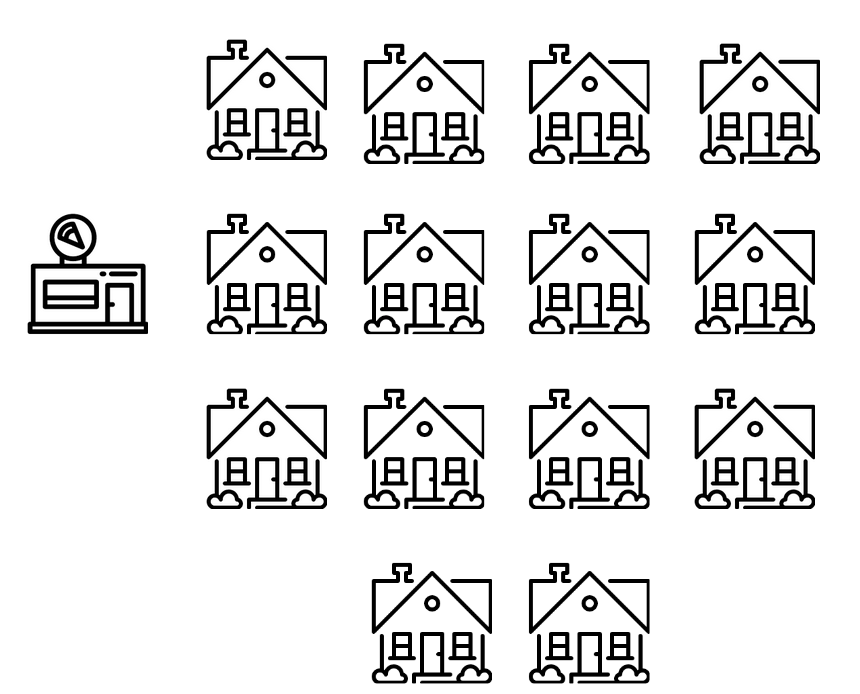
\includegraphics[scale=0.17]{figures/CM0/Pizzeria-1.png}
        \caption{1 pizzeria et 14 maisons}
        \label{fig:piz2}
    \end{figure}
\end{frame}

\begin{frame}{Exemple: la ville et la pizzeria}

    \begin{exampleblock}{Le problème}
    Nous allons considérer 3 villes contenant 14 maisons et 1 pizzeria. Nous souhaitons savoir quelle ville permet aux livreurs de pizza de faire les trajets les plus rapides et pourquoi.
    \end{exampleblock}

    \begin{alertblock}{Temps de calcul}
    On suppose qu'il faut une \alert{unité de temps} pour passer d'une maison à un autre, en suivant une rue.
    \end{alertblock}
    \only<1->{\vspace{-0.3cm}
    \begin{figure}
        \centering
        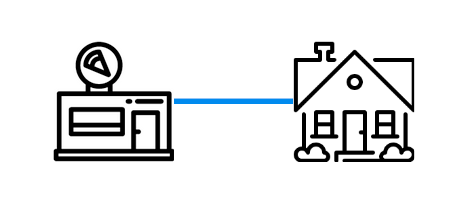
\includegraphics[scale=0.35]{figures/CM0/Pizzeria-Maison.png} 
        \vspace{-0.6cm}
        \caption{Trajet entre la pizzeria et une maison}
    \end{figure}
    }
    \begin{center}
    \uncover<2>{
        \alert{Dans le pire cas, quel est le temps mis par un livreur pour aller de la pizzeria jusqu'à une maison ?}
    }
    \end{center}
\end{frame}


\begin{frame}{Ville A}
\begin{exampleblock}{Organisation de la ville}
Les maisons sont rangées dans l'ordre croissant en ligne droite. La pizzeria se trouve au numéro 1.
\end{exampleblock}
\uncover<2->{
    \begin{figure}
        \centering
        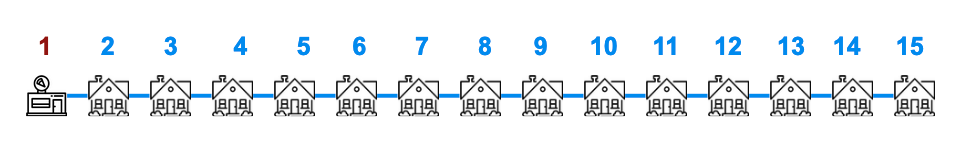
\includegraphics[scale=0.30]{figures/CM0/Pizzeria-2.png}

        \label{fig:piz2}
    \end{figure}
}
\uncover<3->{
    \begin{center}
        Quel est le pire temps possible? \only<4>{\textbf{14}}
    \end{center}
 }  
    
\end{frame}

\begin{frame}{Ville B}
\begin{exampleblock}{Organisation de la ville}
Même organisation que dans la ville A, mais cette fois-ci la pizzeria est au numéro \textbf{8}
\end{exampleblock}
\uncover<2->{
    \begin{figure}
        \centering
        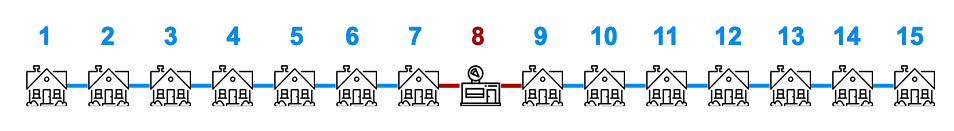
\includegraphics[scale=0.30]{figures/CM0/Pizzeria-3.png}

        \label{fig:piz2}
    \end{figure}
}
\uncover<3->{
    \begin{center}
        Quel est le pire temps possible? \only<4>{\textbf{7}}
    \end{center}
 }  
    
\end{frame}

\begin{frame}{Ville C}
\begin{exampleblock}{Organisation de la ville}
Cette fois-ci, les maisons sont organisées en embranchements, la pizzeria est tout en \textbf{haut}.
\end{exampleblock}
        \begin{figure}
        \centering
        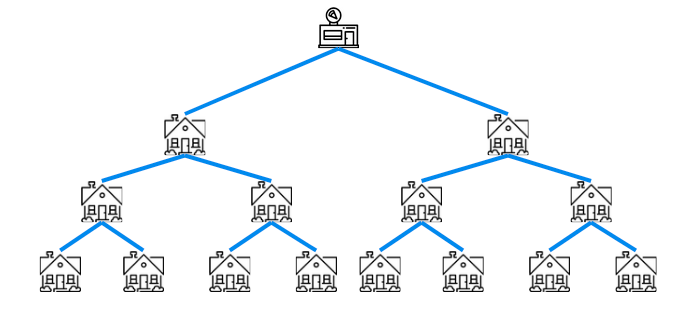
\includegraphics[scale=0.40]{figures/CM0/Pizzeria-4.png}

        \label{fig:piz4}
    \end{figure}
    
    \begin{center}
        \only<1-2>{Quel est le pire temps possible? \only<2>{\textbf{3}}}
        \only<3>{
        \alert{Comment numéroter les maisons ?}
        }
    \end{center}
\end{frame}

\begin{frame}{Ville C : première numérotation}
        \begin{figure}
        \centering
        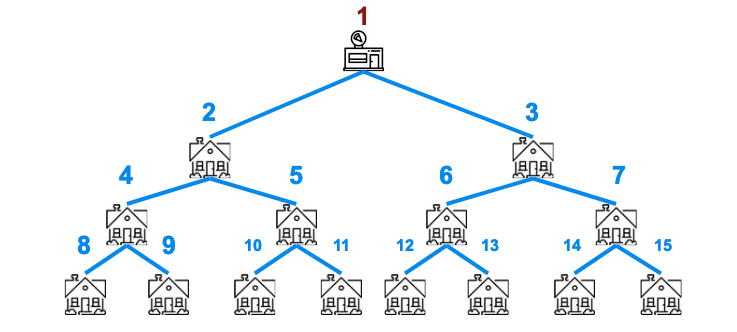
\includegraphics[scale=0.40]{figures/CM0/Pizzeria-5.png}

        \label{fig:piz5}
    \end{figure}
    
    \begin{center}
        \only<2>{
        \alert{Comment choisir la bonne rue à prendre ?}
        }
        
    \end{center}
\end{frame}

\begin{frame}{Ville C : deuxième numérotation}
        \begin{figure}
        \centering
        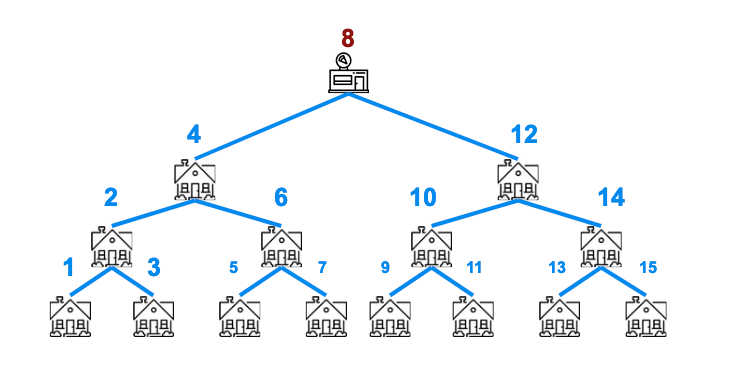
\includegraphics[scale=0.40]{figures/CM0/Pizzeria-6.png}

        \label{fig:piz6}
    \end{figure}
    
    \uncover<2>{
    \begin{center}
        Dans ce cas là, si le numéro de la maison à livrer est plus petit que celui sur lequel on se trouve, on va à gauche, sinon on va à droite.
    \end{center}
    }
\end{frame}


\begin{frame}{Tableau récapitulatif}
    \begin{table}[]
\begin{tabular}{|c|c|c|c|}
\hline
\textbf{Nombre de maisons} &\textbf{Ville A} & \textbf{Ville B} & \textbf{Ville C} \\ \hline
\textbf{15}                & 14                                       & 7                                        & 3                                        \\ \hline
\only<2->{\textbf{1023}              &} \only<3->{1022                                     & 511                                      & 9                                        \\ \hline}
\only<4->{\textbf{n}                 &} \only<5->{n-1                                      &} \only<6->{$\frac{n-1}{2}$                                  &} \only<7->{$\approx log_2(n)$                                 \\ \hline}
\end{tabular}
\end{table}

\end{frame}

\begin{frame}{Et pourquoi pas en étoile ?}
        \begin{figure}
        \centering
        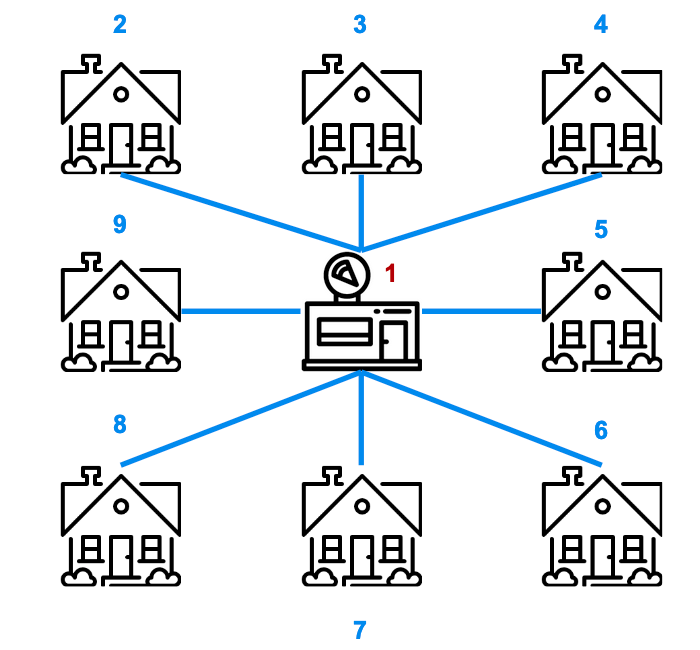
\includegraphics[scale=0.25]{figures/CM0/Pizzeria-etoile.png}

        \label{fig:piz6}
    \end{figure}
    
    \begin{center}
        \only<1>{Cette configuration semble optimale, quel peut être le problème ?}
        \only<2>{Une organisation en étoile avec la pizzeria au milieu permet des trajets très courts, mais \alert{choisir} la bonne rue prend du temps.}
    \end{center}
\end{frame}

\begin{frame}{Complexité: quelques définitions}

\begin{alertblock}{Complexité}
La \textbf{\alert{complexité}} dans le pire cas d'un algorithme est la fonction mathématique $\mathcal{T}$ qui donne le \alert{nombre maximal d'instructions élémentaires} que l'algorithme effectue en fonction de la taille des données manipulées.\\
\end{alertblock}

\begin{exampleblock}{Exemple précédent}
Dans notre exemple précédent, la taille des données manipulées étaient le nombre de maisons.
\end{exampleblock}
\end{frame}

\begin{frame}{Complexité dans le pire cas: À quoi ça sert ?}
    \begin{itemize}
        \item \alert{\textbf{Évaluer le temps d'exécution}} d'un algorithme en fonction de la longueur de l'énoncé;
        \item \alert{\textbf{Comparer les performances}} de différents algorithmes résolvant le même problème;
        \item \alert{\textbf{Évaluer la taille maximale}} des énoncés qu'un algorithme peut traiter;
        \item Mesure du temps \alert{\textbf{indépendante des machines}} puisque l'on compte le nombre d'instructions.
    \end{itemize}
\end{frame}


\begin{frame}{Ordre de grandeur}
Pour comparer des algorithmes, il n'est pas nécessaire d'utiliser la fonction $\mathcal{T}$, mais seulement l'ordre de grandeur asymptotique, noté $\mathcal{O}$ (prononcé "\textit{grand O}").

\begin{alertblock}{Définition formelle}
Une fonction $\mathcal{T}(n)$ est en $\mathcal{O}(f(n))$ ("\textit{en grand O de f(n)}") si:
\begin{equation*}
    \exists n_0 \in \mathbb{N}, \exists c \in \mathbb{R}^+, \forall n \in \mathbb{R}^+, n \geq n_0 \implies | T(n) | \leq c | f(n) | 
\end{equation*}
\end{alertblock}

\only<1>{
Autrement dit, $\mathcal{T}(n)$ est en $\mathcal{O}(f(n))$ s'il existe un seuil $n_0$ à partir duquel la fonction $\mathcal{T}$ est toujours dominée par la fonction $f$, à une constance multiplicative fixée $c$.
}

\end{frame}


\begin{frame}{Quelques exemples}
    \begin{exampleblock}{Exemples}
\begin{itemize}
    \item $T_1(n) = 7 \only<2->{= \mathcal{O}(7)} = \only<3->{\mathcal{O}(1)}$
    \item $T_2(n) = 12n + 5 \only<4->{= \mathcal{O}(12n)} \only<5->{= \mathcal{O}(n)}$
    \item $T_3(n) = 4n^2 + 2n + 6 \only<6->{= \mathcal{O}(4n^2 + 2n)} \only<7->{= \mathcal{O}(n^2)}$
    \item $T_4(n) = 2 + (n-1) \times 5 \only<8->{= \mathcal{O}(n-1)} \only<9->{= \mathcal{O}(n)}$
\end{itemize}
\end{exampleblock}

\uncover<10->{
\begin{exampleblock}{À vous de jouer}
Quelle est la complexité dans le pire des cas des exemples suivants ?
\begin{itemize}
    \item $T_5(n) = 3n + log(n)^4 + 2 \only<11->{= \mathcal{O}(n)}$
    \item $T_6(n) = 1024  \only<12->{= \mathcal{O}(1)}$
    \item $T_7(n) = 2^n + n^{10} \only<13->{= \mathcal{O}(2^n)}$
\end{itemize}
\end{exampleblock}
}

\end{frame}

\begin{frame}{Rappels des règles utiles}
Les quelques règles suivantes permettent de simplifier les complexités en omettant des termes dominés :
\begin{itemize}
    \item Les \alert{coefficients peuvent être omis} : $14n^2$ devient $n^2$;
    \item $n^a$ domine $n^b$ si $a > b$ : par exemple, $n^2$ domine $n$;
    \item Une exponentielle domine un polynôme : $3^n=exp^{nlog3}$ domine $n^5$;
    \item De même un polynôme domine un logarithme : n domine $(log n)^3$. Cela signifie également que, par exemple, $n^2$ domine $n log n$.
\end{itemize}
\end{frame}



\begin{frame}{Reprenons notre pizzeria}

\begin{table}[]
\begin{tabular}{|c|c|c|c|}
\hline
\textbf{Nombre de maisons} &\textbf{Ville A} & \textbf{Ville B} & \textbf{Ville C} \\ \hline
\textbf{15}                & 14                                       & 7                                        & 3                                        \\ \hline
\textbf{1023}              & 1022                                     & 511                                      & 9                                        \\ \hline
\textbf{n}                 & n-1                                      & $\frac{n-1}{2}$                                  & $log_2(n)$                                 \\ \hline

\only<2->{
\red{\textbf{Complexité pour n}}              & \red{$\mathcal{O}(n)$}                                     & \red{$\mathcal{O}(n)$}                                       & \red{$\mathcal{O}(log(n))$ }                                        \\ \hline
}
\end{tabular}
\end{table}   
\begin{center}
    \uncover<3->{
        On voit que les complexités dans le pire cas de la ville A et de la ville B \textbf{sont les mêmes}
    }
\end{center}
\end{frame}

\begin{frame}{Reprenons notre exemple}
    \begin{itemize}
        \item Dans la ville A et B, l'algorithme naturel pour trouver une maison a une complexité linéaire $\mathcal{O}(n)$
        \item Dans la ville C, l'algorithme naturel pour trouver une maison a une complexité logarithmique $\mathcal{O}(log(n))$
        \item L'organisation de la ville C est beaucoup plus efficace pour livrer les pizzas.
    \end{itemize}
    \uncover<2->{
    \begin{center}
        \alert{À quel point est-ce que c'est plus efficace ?}
    \end{center}
    }
\end{frame}

\begin{frame}{Différence entre n et log n}
    \begin{figure}
        \centering
        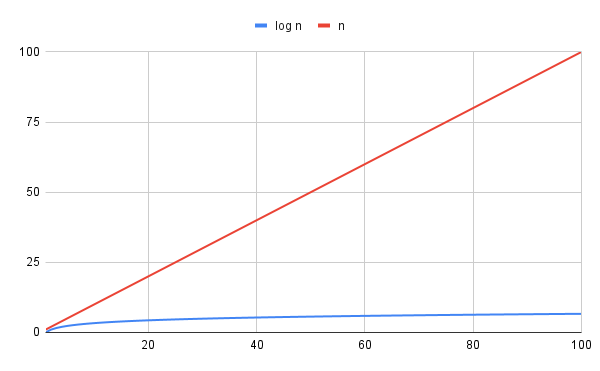
\includegraphics[scale=0.4]{figures/CM0/comp_n_log_n.png}
    \end{figure}
    \begin{itemize}
        \item Si $n = 10^6$, alors $log_2(n) \approx 20 $. Le livreur fait 50 000 fois moins de déplacements si les maisons sont organisées comme dans la ville C.
        
    \end{itemize}
\end{frame}

\begin{frame}{Classe de complexité}
\begin{table}[]
\centering
\begin{tabular}{|c|c|c|c|}
\hline
\textbf{Complexité} & \textbf{Notation}\\
\hline
constante & $\mathcal{O}(1)$ \\
logarithmique &   $\mathcal{O}(log(n))$\\
racinaire &   $\mathcal{O}(\sqrt{x})$ \\
linéaire &    $\mathcal{O}(n)$ \\
quasi-linéaire & $\mathcal{O}(nlog(n))$ \\
quadratique (polynomial) &     $\mathcal{O}(n^2)$ \\
cubique (polynomial) &   $\mathcal{O}(n^3)$ \\
sous-exponentielle &   $\mathcal{O}(2^{poly(log(n))})$ \\
exponentielle &    $\mathcal{O}(2^{poly(n)})$ )\\
factorielle &  $\mathcal{O}(n!)$\\
\hline
\end{tabular}
\captionsetup{justification=centering}
\caption{Évolution du temps de calcul en fonction de la complexité d'un algorithme et de la taille des données}
\label{table:Complexity}
\end{table}

\end{frame}

\begin{frame}{Il existe d'autres complexités}
    \begin{alertblock}{Complexité en moyenne}
    \begin{itemize}
        \item Il s'agit de la complexité en moyenne sur toutes les entrées;
        \item Intéressant car certains problèmes ont une complexité dans le pire cas très élevées, mais les entrées qui correspondent à ces cas ne se produisent que très rarement en pratique;
        \item Étudié essentiellement dans les algorithmes de tri (que nous verrons plus tard)
    \end{itemize}
    \end{alertblock}
    
        \begin{alertblock}{Complexité en mémoire}
    \begin{itemize}
        \item On souhaite ici mesurer la mémoire utilisée par un algorithme;
        \item Certains algorithmes sont en effet très rapide mais prennent beaucoup d'espace mémoire (ou inversement);
    \end{itemize}
    \end{alertblock}
%     
%     \begin{center}
%         Il existe plusieurs autres complexités mais qui ne nous concernent pas directement.
%     \end{center}
\end{frame}

\section{Langage de Description Algorithmique}


% \begin{frame}{Écriture en pseudo code}
%  
%  
% \end{frame}



\begin{frame}{Plus grand diviseur commun (pgcd)}
  \underline{Problème}:
  \begin{itemize}
  \item Entrées: 2 entiers $a>b \geq 0$
  \item Sortie: le  pgcd de $\mathbf{a}$ et $\mathbf{b}$
  \end{itemize}
  Exemple: $     pgcd(123,82) = 41$  \\~\\
  ~\\\uncover<2->{\underline{Opérations élémentaires}: $+,\times,-$ et division euclidienne\\~\\}
  
  \uncover<3->{$
    \noindent\underline{\mbox{Observation}}: \left\{
      \begin{array}{ll}
        pgcd(a,b) & =  pgcd(b,r)  \ \ \mbox{r reste de la div. de a par b} \\
        pgcd(a,0) & = a
      \end{array} \right.
  $
  ~\\~\\Exemple: $pgcd(123,82) = pgcd(82,41) = pgcd(41,0) = 41$}
\end{frame}

\begin{frame}{Pgcd: écriture d'un algorithme}

\textbf{Écriture en pseudo code}\\[2ex]

  $\noindent\underline{\mbox{Observation}}: \left\{
      \begin{array}{ll}
        pgcd(a,b) & =  pgcd(b,r) \ \ \mbox{r reste de la div. de a par b}\\
        pgcd(a,0) & = a \\
      \end{array} \right.
  $\\[2ex]
\underline{Algorithme}: \only<1>{???}
\begin{tabbing}
  aaa\=aaa\=\kill
  \only<7->{\textbf{pgcd}(a,b) \hfill $~~~~~~~~~~~~~~~~~~$\texttt{/* a,b entiers, $a>b \geq 0$ */}}  \\
  \> \only<2->{ \textbf{si} $b=0$ \textbf{retourner} $a$ \textbf{fin si}} \\
  \> \only<3->{ $x \leftarrow a; y \leftarrow b$} \\
  \> \only<6->{\textsl{répéter}} \\
  \> \> \only<3->{$r \leftarrow$ reste de la div. euclidienne de $x$ par $y$} \\
  \> \> \only<4->{\textbf{si} $r = 0$ \textbf{alors} \textbf{retourner} $y$} \\
  \> \> \only<5->{\textbf{sinon} $x \leftarrow y$; $y\leftarrow r$} \\
  \> \> \only<5->{\textbf{fin si}} \\
  \> \only<6->{\textsl{fin répéter}} 
  \end{tabbing}
\end{frame}

\begin{frame}{Algorithme d'Euclide}
  \begin{minipage}{0.45\linewidth}
    \begin{tabbing}
      aaa\=aaa\=\kill
      \textbf{pgcd}(a,b) \\%\hfill $~~~~~~~~~~~~~~~~~~$\texttt{/* a,b entiers, $a>b \geq 0$ */}  \\
      \>  entier $x,y,r$  \\
 \> \only<2->{ \textbf{si} $b=0$ \textbf{retourner} $a$ \textbf{fin si}} \\
      \> \only<2>{$\red{\mathbf{x \leftarrow a; y \leftarrow b}}$} \only<1,3->{$x \leftarrow a; y \leftarrow b$} \\ 
      \> \textbf{tant que} \only<1-17,19->{$y \neq 0$}\only<18>{$\red{\mathbf{y \neq 0}}$} \textbf{faire} \\
       \> \> \only<3,6,9,12,15>{$\red{\mathbf{r\leftarrow x ~\%~ y}}$} \only<1-2,4-5,7-8,10-11,13-14,16->{$r \leftarrow x ~\%~ y$} \\
       \> \> \only<4,7,10,13,16>{$\red{\mathbf{x \leftarrow y}}$}      \only<1-3,5-6,8-9,11-12,14-15,17->{$x \leftarrow y$}\\
       \> \> \only<5,8,11,14,17>{$\red{\mathbf{y\leftarrow r}}$}       \only<1-4,6-7,9-10,12-13,14-15,18->{$y \leftarrow r$}\\
       \> \textbf{fin tant que} \\
      \> \only<1-18>{\textbf{retourner}($x$)}\only<19>{\red{\textbf{retourner}}($\red{\mathbf{x}}$)}
    \end{tabbing}
  \end{minipage}\hfill
  \begin{minipage}{0.45\linewidth}
    \textbf{pgcd}(12345678,123456) \\
     \begin{tabular}{l|l|l}
       r & x & y \\
       \hline
       \only<2->{$\bot$} & \only<2->{12345678}   & \only<2->{123456} \\
       \only<3->{78} 	 & \only<4->{123456} 	 & \only<5->{78} \\
       \only<6->{60} 	 & \only<7->{78} 	 & \only<8->{60} \\
       \only<9->{18} 	 & \only<10->{60} 	 & \only<11->{18} \\
       \only<12->{6} 	 & \only<13->{18} 	 & \only<14->{6} \\ 
       \only<15->{0} 	 & \only<16-18>{6}\only<19>{\red{\textbf{6}}} 	 & \only<17->{0} \\
       \end{tabular}
\end{minipage}
\end{frame}






\section{Algorithmes Récursifs}


\begin{frame}{Rappels}
    \begin{alertblock}{Complexité d'un algorithme}
    \begin{itemize}
        \item La complexité permet d'évaluer l'efficacité d'un algorithme;
        \item Elle permet de comparer des algorithmes indépendamment des machines;
        \item On note $\mathcal{O}$ la complexité asymptotique (\textit{dans le pire cas}).
    \end{itemize}
    \end{alertblock}
\end{frame}


\begin{frame}{Introduction}
    \begin{itemize}
        \item Les \alert{\textbf{algorithmes récursifs}} et les \alert{\textbf{fonctions récursives}} sont fondamentaux en informatique. Un algorithme est dit récursif s'il s'appelle \textbf{lui-même};
        \item Les premiers langages de programmation qui ont introduit la récursivité sont \texttt{LISP} et \texttt{Algol 60} et maintenant tous les langages de programmation modernes proposent une implémentation de la récursivité;
        \item On oppose généralement les algorithmes récursifs aux algorithmes dits \alert{impératifs} ou \alert{itératifs} qui s'exécutent sans invoquer ou appeler explicitement l'algorithme lui-même.
    \end{itemize}
\end{frame}



\begin{frame}{Lien avec les mathématiques : la factorielle}
On souhaite calculer $n!$. On rappelle que pour tout entier $n \geq 0$

\begin{equation*}
    n! = \prod_{i=1}^{n} i = 1 \times 2 \times \ldots \times n
\end{equation*}

\uncover<2->{On peut déduire de cette définition la propriété importante suivante

\begin{equation*}
    \forall n \geq 1, n! = n \times (n - 1)!
\end{equation*}

et donc si on sait calculer (n-1)! alors on sait calculer n!.
}

\uncover<3->{
Par ailleurs, on sait que 0! = 1. On sait donc calculer 1!, puis 2!, et par récurrence on peut établier qu'on sait calculer n! pour tout entier $n \geq 0$.
}
\end{frame}



\begin{frame}{Algorithme de la factorielle}
L'algorithme récursif de calcul de la factorielle distingue deux cas. Le premier cas ne nécessite aucun calcul, le second utilise la fonction $fact$ pour calculer $(n-1)!$

\begin{tcolorbox}
  \begin{algorithmic}[1]
    \Function{fact}{$n$}
      \If{ n == 0 }
        \State\text{\textbf{return}} 1
      \Else
        \State\text{\textbf{return}} $n \times fact(n-1)$
      \EndIf
    \EndFunction
  \end{algorithmic}
\end{tcolorbox}

\end{frame}

\begin{frame}{Exécution de l'algorithme de la factorielle}

Prenons l'exemple du déroulement du calcul récursif de $4!$ :
\begin{center}
    \begin{itemize}[<+->]
\item[] $fact(4) \rightarrow 4 \times fact(3)$
\item[] $fact(4) \rightarrow 4 \times 3 \times fact(2)$
\item[] $fact(4) \rightarrow 4 \times 3 \times 2 \times fact(1)$
\item[] $fact(4) \rightarrow 4 \times 3 \times 2 \times 1 \times fact(0)$
\item[] $fact(4) \rightarrow 4 \times 3 \times 2 \times 1 \times 1$
\item[] $fact(4) \rightarrow 24$
\end{itemize}
\end{center}
\end{frame}

\begin{frame}{Autre algorithme de factorielle}
    Considérons l'algorithme suivant :
    
    \begin{tcolorbox}
  \begin{algorithmic}[1]
    \Function{$fact2$}{$n$}
        \State\text{\textbf{return}} $n \times fact(n-1)$
    \EndFunction
  \end{algorithmic}
\end{tcolorbox}

\uncover<2->{\alert{Quel est le soucis avec cette fonction ?}}

\uncover<3->{L'évaluation de $fact2(1)$ conduit à un calcul infini:}
\end{frame}

\begin{frame}{Exécution de l'algorithme de la factorielle}

Prenons l'exemple du déroulement du calcul récursif de $4!$:
\begin{center}
    \begin{itemize}[<+->]
\item[] $fact2(1) \rightarrow 1 \times fact2(0)$
\item[] $fact2(1) \rightarrow 1 \times 0 \times fact2(-1)$
\item[] $fact2(1) \rightarrow 1 \times 0 \times -1 \times fact2(-2)$
\item[] $fact2(1) \rightarrow \ldots $
\end{itemize}
\end{center}

\end{frame}


\begin{frame}{Règle implicite de conception d'un algorithme récursif}
    \begin{exampleblock}{Règle implicite}
        Tout algorithme récursif doit distinguer plusieurs cas dont l'un au moins ne doit pas contenir d'appels récursifs.
    \end{exampleblock}
    
    Les cas non récursifs d'un algorithme récursif sont appelés \alert{\textit{cas de bases}}. Les conditions que doivent satisfaire les données dans ces cas de bases sont appelées \alert{\textit{conditions de terminaison}}.
    
    \uncover<2>{\begin{center}
        \alert{Est-ce-que c'est suffisant ?}
    \end{center}  }
\end{frame}

\begin{frame}{Reprenons notre exemple de la factorielle}
    
    \begin{tcolorbox}
  \begin{algorithmic}[1]
    \Function{fact3}{$n$}
      \If{ n == 0 }
        \State\text{\textbf{return}} 1
      \Else
        \State\text{\textbf{return}} $n \times fact3(n+1)$
      \EndIf
    \EndFunction
  \end{algorithmic}
\end{tcolorbox}
    \uncover<2->{\alert{Quel est le soucis avec cette fonction ?}}

    \uncover<3->{L'évaluation de $fact3(1)$ conduit à un calcul infini:
}
\end{frame}

\begin{frame}{Exécution de l'algorithme de la factorielle}

Prenons l'exemple du déroulement du calcul récursif de $4!$:
\begin{center}
    \begin{itemize}[<+->]
\item[] $fact3(1) \rightarrow 1 \times fact3(2)$
\item[] $fact3{1} \rightarrow 1 \times 2 \times fact3(3)$
\item[] $fact3{1} \rightarrow 1 \times 2 \times 3 \times \ldots$
\end{itemize}
\end{center}

\end{frame}

\begin{frame}{Deuxième règle implicite}
        \begin{tcolorbox}
  \begin{algorithmic}[1]
    \Function{fact3}{$n$}
      \If{ n == 0 }
        \State\text{\textbf{return}} 1
      \Else
        \State\text{\textbf{return}} $n \times fact3(n+1)$
      \EndIf
    \EndFunction
  \end{algorithmic}
\end{tcolorbox}
\uncover<2>{
\begin{exampleblock}{Deuxième règle}
À chaque appel récursif il faut se rapprocher des conditions de terminaison.
\end{exampleblock}
}
\end{frame}



% \begin{frame}{Un autre exemple: les tours de Hanoï}
%     \begin{alertblock}{Principe du jeu}
%     \begin{itemize}
%         \item On dispose de 3 tours côte à côte sur lesquelles on peut empiler des disques de diamètre croissant;
%         \item On ne peut déplacer qu'un disque à la fois et on ne doit pas poser un disque plus large sur un plus petit;
%         \item L'objectif est de trouver la suite de déplacements qui permet de placer tous les disques sur la tour la plus à droite.
%     \end{itemize}
%     \end{alertblock}
%     
%     \begin{figure}
%         \centering
%         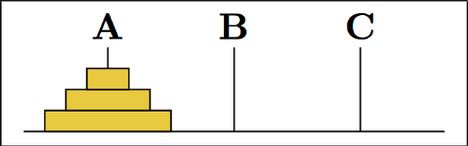
\includegraphics[scale=0.4]{figures/CM1/Hanoi-initial.png}
%         \label{fig:my_label}
%     \end{figure}
%     \uncover<2>{\centering \alert{À vous de jouer ! En combien de mouvements est-ce possible ?}}
% \end{frame}
% 
% \begin{frame}{Résolution du problème de Hanoï}
%     \only<1->{\centering \alert{\textbf{La réponse: 7 !}}}
%     \only<2->{\begin{figure}
%         \centering
%         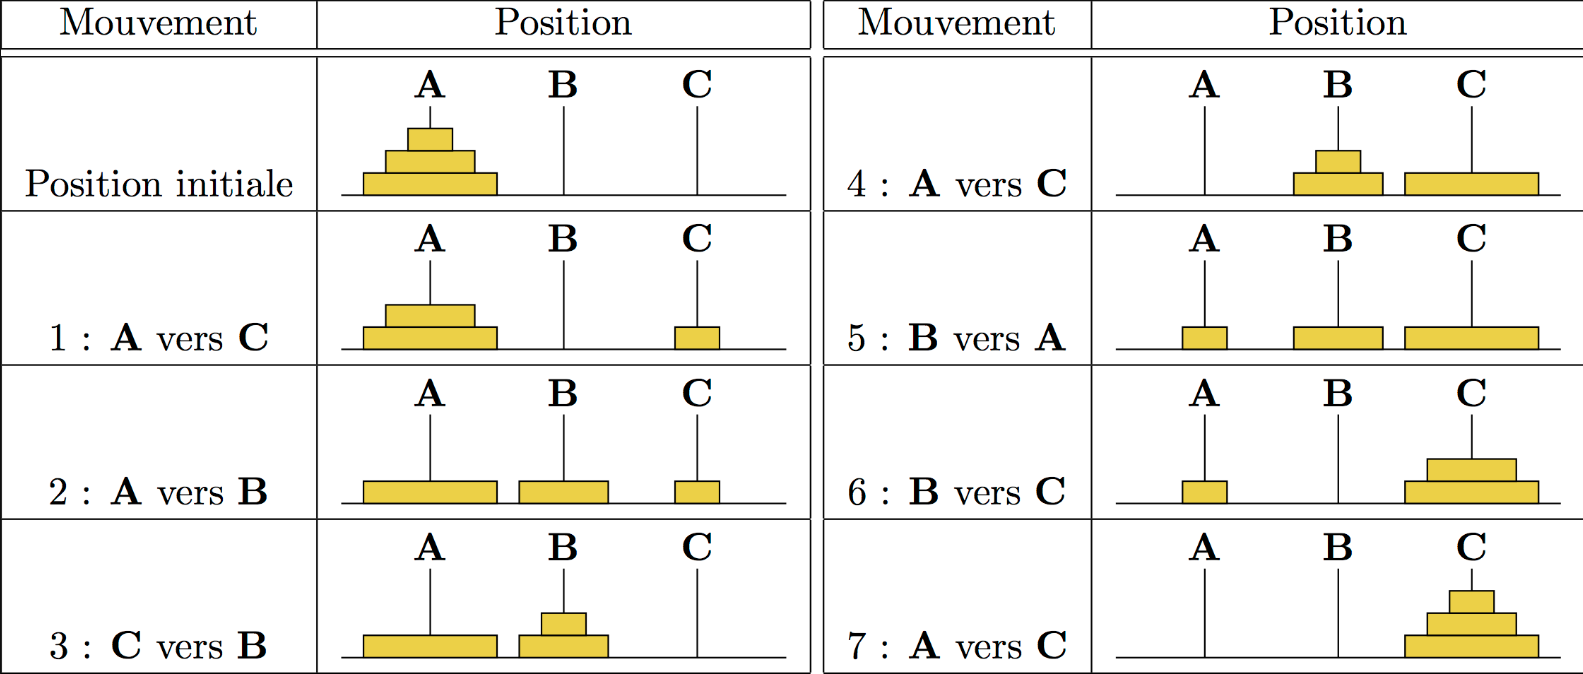
\includegraphics[scale=0.18]{figures/CM1/Hanoi.png}
% 
%         \label{fig:my_label2}
%     \end{figure}
%     }
% \uncover<3>{\centering \alert{Quel est l'algorithme ?}}
% \end{frame}
% 
% \begin{frame}{Algorithme de résolution des tours de Hanoï dans le cas général}
%     Cet algorithme est la fonction $hanoi$ qui prend trois paramètres:
%     \begin{enumerate}
%         \item \alert{n} le nombre de disques à déplacer;
%         \item \alert{d} la tour de départ où se trouvent ces disques;
%         \item \alert{a} la tour d'arrivée où doivent aller les disques
%     \end{enumerate}
%     On suppose que l'on a une fonction $deplacerdisque(d,a)$ qui permet de déplacer un disque de $d$ jusqu'à $a$.
%     \uncover<2>{  
%         \begin{tcolorbox}
% 
%   \begin{algorithmic}[1]
%     \Function{hanoi}{$n,d,a$}
%       \If{ $n > 0 $}
%         \Let{$aux$}{$\text{le piquet différent de d et a}$}
%         \State $hanoi(n - 1, d, aux)$
%         \State $deplacerdisque(d,a)$
%         \State $hanoi(n - 1, aux, a)  $
%       \EndIf
%     \EndFunction
%   \end{algorithmic}
% \end{tcolorbox}
% }
% \end{frame}

\begin{frame}{Petit exercice}
    \begin{alertblock}{Exercice}
    Écrire une fonction qui calcule la somme des inverses des carrés des $n$ premiers entiers naturels non nuls.
    \end{alertblock}
    \uncover<2>{
    
    \begin{tcolorbox}

  \begin{algorithmic}[1]
    \Function{$sum\_inv$}{$n$}
      \If{ $n == 0 $}
          \State \textbf{return} 1
      \Else
          \State \textbf{return} $1/n^2 + sum\_inv(n-1)$
      \EndIf
    \EndFunction
  \end{algorithmic}
\end{tcolorbox}
    }
\end{frame}

% \section{Type de récursivité}
% 
% \begin{frame}{Récursivité simple ou linéaire}
%     Un algorithme récursif est \textit{simple} ou \textit{linéaire} si chaque cas qu'il distingue se résout en au plus un appel récursif.
%     
% \begin{tcolorbox}
% 
%   \begin{algorithmic}[1]
%     \Function{mystere}{$n$}
%       \If{ $n == 0 $}
%          \State\text{\textbf{return}} 1
%        \Else
%        \State\text{\textbf{return}} $mystere(n - 1) \times 2$
%       \EndIf
%     \EndFunction
%   \end{algorithmic}
%   
% \end{tcolorbox}
% 
% \uncover<2>{\centering \alert{Que fait cet algorithme ?}}
%     
% \end{frame}
% 
% 
% \begin{frame}{Récursivité terminale}
% \uncover<1-4>{Une définition de fonction f est récursive terminale quand tout appel récursif est de la forme return f(...); La valeur retournée est directement la valeur obtenue par un appel récursif, sans qu'il n'y ait aucune opération sur cette valeur.
% }
%  \vspace{-0.05cm}
% \uncover<2->{
% \begin{tcolorbox}
% 
%   \begin{algorithmic}[1]
%     \Function{$recursionTerminale$}{$n$}
%          \State\text{\textbf{...}} 
%        \State\text{\textbf{return}} $recursionTerminale(n - 1)$
%     \EndFunction
%   \end{algorithmic}
%  \end{tcolorbox}
%  
%  }
%  
%  \vspace{-0.05cm}
%  
%  \uncover<3->{
%  \begin{tcolorbox}
%     \begin{algorithmic}[1]
%     \Function{$recursionNonTerminale$}{$n$}
%          \State\text{\textbf{...}} 
%        \State\text{\textbf{return}} $n + recursionTerminale(n - 1)$
%     \EndFunction
%   \end{algorithmic}
%   
% \end{tcolorbox}
% }
%  \vspace{-0.2cm}
% \uncover<4->{
% Dans le premier cas, aucune référence aux résultats précédents n'est à conserver en mémoire, tandis que dans le second cas, tous les résultats intermédiaires doivent l'être.
% }
% \end{frame}
% 
% \begin{frame}{Et la fonction factorielle ?}
%     Reprenons la fonction $factorielle$
%     \begin{tcolorbox}
%   \begin{algorithmic}[1]
%     \Function{fact}{$n$}
%       \If{ n == 0 }
%         \State\text{\textbf{return}} 1
%       \Else
%         \State\text{\textbf{return}} $n \times fact(n-1)$
%       \EndIf
%     \EndFunction
%   \end{algorithmic}
% \end{tcolorbox}
%     \uncover<2->{\centering \alert{Est-elle récursive terminale ?}}
%     \uncover<3>{\centering \alert{Non, il y a une multiplication par n avant de retourner.}}
% \end{frame}
% 
% \begin{frame}{Exemple d'une fonction récursive terminale}
%         \begin{tcolorbox}
%   \begin{algorithmic}[1]
%     \Function{f}{$n,a$}
%       \If{ n <= 1 }
%         \State\text{\textbf{return}} a
%       \Else
%         \State\text{\textbf{return}} $f(n-1,n*a)$
%       \EndIf
%     \EndFunction
%   \end{algorithmic}
% \end{tcolorbox}
%      \uncover<2->{\centering \alert{Que fait cette fonction ?}}
% \end{frame}
% 
% \begin{frame}{Avantage de la récursivité terminale}
%     \begin{itemize}
%         \item     La plupart des langages fonctionnels (comme \textit{LISP} et \textit{CAML}) exécutent un programme à récursivité terminale comme s'il était itératif, c'est-à-dire en espace constant.
%         \item Une fonction récursive terminale peut toujours être transformée en itération.
%     \end{itemize}
% 
% 
% \end{frame}
% 
% \begin{frame}{Petit exercice}
%     \begin{alertblock}{Transformer cette fonction récursive terminale en itération}
%                 \begin{tcolorbox}
%   \begin{algorithmic}[1]
%     \Function{f}{$n,a$}
%       \If{ n <= 1 }
%         \State\text{\textbf{return}} a
%       \Else
%         \State\text{\textbf{return}} $f(n-1,n*a)$
%       \EndIf
%     \EndFunction
%   \end{algorithmic}
% \end{tcolorbox}
%     \end{alertblock}
%     
%     \uncover<2>{
%     \begin{tcolorbox}
%   \begin{algorithmic}[1]
%     \Function{f}{$n$}
%       \Let{$a$}{$1$}
%       \While{ n > 1 }
%         \Let{$a$}{$n*a$}
%         \Let{$n$}{$n-1$}
%       \EndWhile
%         \State\text{\textbf{return}} $a$
% 
%     \EndFunction
%   \end{algorithmic}
% \end{tcolorbox}
%     
%     }
% \end{frame}
% 
% \begin{frame}{Récursivité multiple}
% \begin{exampleblock}{Définition}
%         Un algorithme récursif est multiple si l’un des cas qu’il distingue se résout avec plusieurs appels récursifs.
% \end{exampleblock}
% Prenons la suite de fibonacci comme exemple
% 
% \begin{equation}
%                 fibo(n)=\begin{cases} 1 &, \text{si $n=0$}.\\ 1 &, \text{si $n=1$}.\\ fibo(n-1) + fibo(n-2) &, \text{si $n>1$}. \end{cases} 
% \end{equation}
% \end{frame}
% 
% 
% 
% \begin{frame}{Récursivité croisée}
%     \begin{exampleblock}{Définition}
% Deux algorithmes sont dits mutuellement récursifs si l’un fait appel à l’autre et l’autre à l’un. On parle aussi de récursivité croisée.
% \end{exampleblock}
% 
% \begin{tcolorbox}
%   \begin{algorithmic}[1]
%     \Function{pair}{$n$}
%         \If{$n == 0$}
%         \State \textbf{return} True
%         \Else
%         \State \textbf{return} $impair(n - 1)$
%         \EndIf
%     \EndFunction
%   \end{algorithmic}
%   
%     \begin{algorithmic}[1]
%     \Function{impair}{$n$}
%         \If{$n == 0$}
%         \State \textbf{return} False
%         \Else
%         \State \textbf{return} $pair(n - 1)$
%         \EndIf
%     \EndFunction
%   \end{algorithmic}
% \end{tcolorbox}
% 
% \end{frame}


\section{Recherche dans un tableau}

\begin{frame}{Algorithme de recherche d'un élément dans un tableau}
    \begin{tcolorbox}
  \begin{algorithmic}[1]
    \Function{search}{$tab,e$}
        \For{$i < tab.size$}
        
        \If{$tab[i] == e$}
            \State \textbf{return} $i$
        \EndIf
    \EndFor
    \State \textbf{return} nonTrouvé
    \EndFunction
  \end{algorithmic}
\end{tcolorbox}

\uncover<2->{\centering \alert{Quelle est la complexité de cette fonction ?}} 
\uncover<3>{$\mathcal{O}(n)$}

\end{frame}

\begin{frame}{Recherche d'un élément dans un tableau}
    La complexité précédente est trop élevée, surtout sachant que la recherche dans un tableau est une opération de base utilisée dans de nombreux algorithmes.\\
    
    Pour aller plus vite, on peut utiliser les \textbf{tableaux triés} et la \textbf{dichotomie}.
\end{frame}

  
\begin{frame}{Exemple : La dichotomie}
    \begin{exampleblock}{Definition}
    La recherche dichotomique, ou recherche par dichotomie (en anglais : \textit{binary search}), est un algorithme de recherche pour trouver la position d'un élément dans un tableau trié.
    \end{exampleblock}
\begin{alertblock}{Le principe}
L'objectif est trouver la position d'un élément dans un tableau trié.
\begin{itemize}
    \item On trouve l'élément $m$ avec la position la plus centrale du tableau (si le tableau est vide on s'arrête);
    \item On compare la valeur de l'élément recherché avec l'élément $m$;
    \item Si elle est plus petite, on recommence dans le sous-tableau de gauche, sinon dans le sous-tableau de droite.
\end{itemize}
\end{alertblock}

\end{frame}

\begin{frame}{L'algorithme de la dichotomie}
    
\begin{tcolorbox}
  \begin{algorithmic}[1]
    \Function{dichotomie}{$tab,min,max,e$}
        
        \If{$min == max$}
            \If{$tab[min] = e$}
                \State \textbf{return} $min$
        \Else
            \State \textbf{return} nonTrouvé
                        \EndIf
        \EndIf
    \Let{$mid$}{$( min + max ) / 2$}
    \If{$tab[mid] < e$}
        \State \textbf{return} $dichotomie(tab, mid+1, max, e)$
    \Else
        \State \textbf{return} $dichotomie(tab, min, mid, e)$
    \EndIf
    \EndFunction
  \end{algorithmic}
\end{tcolorbox}

\uncover<2->{\centering \alert{Quelle est la complexité de cette fonction ?}} 
\uncover<3>{$\mathcal{O}(log_2(n))$}

\end{frame}

\begin{frame}{L'algorithme de la dichotomie itérative}
    
\begin{tcolorbox}
  \begin{algorithmic}[1]
    \Function{dichotomie}{$tab,e$}
    \Let{$min$}{$0$}
    \Let{$max$}{$\text{taille - 1}$}
    \While{$min < max$}
        \Let{$mid$}{$( min + max ) / 2 $}
        \If{$tab[mid] < e$}
            \Let{$min$}{$mid+1$}
        \Else
            \Let{$max$}{$mid$}
        \EndIf
    \EndWhile 
    \If{$\text{tab[min] == e}$}
        \State \textbf{return} $min$
    \Else
        \State \textbf{return} nonTrouvé
    \EndIf
    \EndFunction
  \end{algorithmic}
\end{tcolorbox}

\vspace{-0.2cm}

\uncover<2->{\centering \alert{Quelle est la complexité de cette fonction ?}} 
\uncover<3>{$\mathcal{O}(log_2(n))$}

\end{frame}


\begin{frame}{Complexité de la Recherche Dichotomique}
  \begin{minipage}{.3\linewidth}
    \begin{tikzpicture}[invis/.style={draw=none}]
    \tikzstyle{level 1}=[edge from parent/.style={draw}, sibling distance=17mm]
    \tikzstyle{level 3}=[edge from parent/.style={draw,dashed}, sibling distance=17mm]
    \tikzstyle{level 5}=[edge from parent/.style={draw=none}, sibling distance=17mm]
    \tikzstyle{level 10}=[edge from parent/.style={draw=none}, level distance=5mm]
    \tikzstyle{level 11}=[edge from parent/.style={draw=none}, level distance=15mm]
    \tikzstyle{every node}=[fill=white,rectangle, rounded corners,draw=black,solid,minimum width=14mm]
    \tikzstyle{every node}=[fill=white,rectangle, rounded corners,draw=black,solid,minimum width=14mm]
    \node {$n$}
    child {node {$n/2$}
      child {node {$n/4$}
        child {node {$n/2^k$}
          child {node {$1$}
            child[grow=right] {node[invis] {$\log_2 n$}
              child[grow=up] {node[invis] {$k$}
                child[grow=up] {node[invis] {2}
                  child[grow=up] {node[invis] {1}
                    child[grow=up] {node[invis] {0}
                      child[grow=up] {node[invis] {niveaux}
                        child[grow=left] {node[invis] {taille}
                        }
                      }
                  }
                }
              }
            }
          }
        }
      }
    }
};
  \end{tikzpicture}
\end{minipage}
\hfill\begin{minipage}[r]{.6\linewidth}
  \only<2->{Niveau $k$}
  \begin{itemize}
  \item<2-> $\mathbf{1}$ sous problème de taille $\mathbf{n/2^k}$
  \item<2-> $\mathcal{O}(1)$ opérations élémentaires  par niveau
  \end{itemize}
  \uncover<3->{Total:}
  \begin{itemize}
  \item<3-> taille du problème divisée par 2 à chaque niveau $\implies \log_2 n +1$ niveaux.
  \item<4-> \underline{Complexité} = $\mathcal{O}(\log n)$
\end{itemize}
\end{minipage}
\end{frame}

% \begin{frame}{Exercice}
%     \begin{exampleblock}{Exercice}
%         Déterminer la version itérative de l'algorithme de la dichotomie
%     \end{exampleblock}
% \end{frame}
% 
% \begin{frame}{L'algorithme de la dichotomie itérative (variante)}
% 
% \begin{tcolorbox}
%   \begin{algorithmic}[1]
%     \Function{dichotomie}{$tab,e$}
%     \Let{$min$}{$0$}
%     \Let{$max$}{$\text{taille - 1}$}
%     \While{$min < max$}
%         \Let{$mid$}{$( min + max ) / 2 $}
%         \If{$tab[mid] == e$}
%             \State \textbf{return} $mid$
%         \EndIf
%         \If{$tab[mid] < e$}
%             \Let{$min$}{$mid+1$}
%         \Else
%             \Let{$max$}{$mid$}
%         \EndIf
%     \EndWhile 
%     \If{$tab[min] == e$}
%         \State \textbf{return} $min$
%     \Else
%         \State \textbf{return} nonTrouvé
%     \EndIf
%     \EndFunction
%   \end{algorithmic}
% \end{tcolorbox}
% 
% \vspace{-0.2cm}
% 
% \uncover<2->{\centering \alert{Quelle est la complexité de cette fonction ?}} 
% \uncover<3>{$\mathcal{O}(log_2(n))$}
% 
% 
% \end{frame}

\begin{frame}{Autres applications de la recherche dichotomique}

\begin{itemize}
    \item Jeu du nombre inconnu où l'on répond soit "plus grand" soit "plus petit" soit "gagné";
    \item Calcul d'une racine d'une fonction croissante;
    \item Algorithme de pointage et de visée;
    \item Recherche de l'apparition d'un bug dans l'histoire d'un programme.
\end{itemize}
\end{frame}

\section{Tri de tableaux et algorithmes de tris}

\begin{frame}{Insertion dans un tableau trié}
    \begin{tcolorbox}
  \begin{algorithmic}[1]
    \Function{Insertion}{$tab,e$}
    \Let{$i$}{$taille$}

    \While{$\text{i > 0 and tab[i - 1] > e}$}
        \Let{$tab[i]$}{$tab[i - 1]$}
        \Let{$i$}{$i - 1$}
    \EndWhile
    \Let{$tab[i]$}{$e$}
    \Let{$taille$}{$taille + 1$}
    \EndFunction
  \end{algorithmic}
\end{tcolorbox}

\uncover<2->{\centering \alert{Quelle est la complexité de cette fonction ?}} 
\uncover<3>{$\mathcal{O}(n)$}

\end{frame}

\begin{frame}{Tri par insertion}
    \begin{tcolorbox}
  \begin{algorithmic}[1]
    \Function{Insertsort}{$tab$}
    \Let{$i$}{$1$}
    \For{$i < taille$}
        \Let{$e$}{$tab[i]$}
        \Let{$j$}{$i$}
        \While{$\text{j > 0 and tab[j - 1] > e}$}
            \Let{$tab[j]$}{$tab[j - 1]$}
            \Let{$j$}{$j - 1$}
        \EndWhile
        \Let{$tab[j]$}{$e$}
    \EndFor
    \EndFunction
  \end{algorithmic}
\end{tcolorbox}

\uncover<2->{\centering \alert{Quelle est la complexité de cette fonction ?}}
\uncover<3>{$\mathcal{O}((n^2))$}

\end{frame}



\section{Diviser pour régner}
\begin{frame}{Approche diviser pour régner}
En informatique, \textbf{\alert{diviser pour régner}} est une technique algorithmique consistant à : 
  \begin{enumerate}
  \item \alert{Diviser} : découper un problème initial en sous-problèmes;
  \item \alert{Régner} : résoudre les sous-problèmes (récursivement ou directement s'ils sont assez petits);
  \item \alert{Combiner} : calculer une solution au problème initial à partir des solution des sous-problèmes.
  \end{enumerate}
  
 \uncover<2>{\alert{\textbf{Comment obtenir un tableau trié, si l'on sait trier chaque moitié ?}}}

  \end{frame}
 
 
 \begin{frame}{Fusion de tableaux triés}
            \begin{tcolorbox}
  \begin{algorithmic}[1]
    \Function{$fusion$}{$A[a_1,a_2,\ldots,a_n],B[b_1,b_2,\ldots,b_n]$}
        \If{$\text{A est vide}$}
            \State \textbf{return} B
        \EndIf
        \If{$\text{B est vide}$}
            \State \textbf{return} A
        \EndIf
        \If{$A[a_1] <= B[b_1]$}
            \State \textbf{return} A[$a_1$] + fusion($A[a_2,\ldots,a_n],B$)
        \Else
            \State \textbf{return} B[$b_1$] + fusion($A, B[b_2,\ldots,b_n]$)   
        \EndIf
    \EndFunction
  \end{algorithmic}
\end{tcolorbox}


     \uncover<2->{\centering \alert{Quelle est la complexité de cette fonction ?}} 
     \uncover<3>{$\mathcal{O}((t_a + t_b))$}
     
 \end{frame}

\begin{frame}{Tri par fusion (MergeSort)}
                \begin{tcolorbox}
  \begin{algorithmic}[1]
    \Function{$trifusion$}{$T[t_1,t_2,\ldots,t_n]$}
        \If{$t_n <= 1$}
            \State \textbf{return} T
        \Else
            \State \textbf{return} fusion(triFusion(T[$t_1, \ldots, t_{n/2}$]), triFusion(T[$t_{n/2 + 1}, \ldots, t_n$]))
        \EndIf
    \EndFunction
  \end{algorithmic}
\end{tcolorbox}

     \uncover<2->{\centering \alert{Quelle est la complexité de cette fonction ?}} 
     \uncover<3>{$\mathcal{O}(nlogn)$}
\end{frame}



\section{Implémentation en C}


\begin{frame}[fragile,label=nnn]{Variable aléatoire}
 
{\small
 La fonction \ttt{rand} (\ttt{\#include<stdlib.h>})
 retourne un entier pseudo-aléatoire : \\[0.25ex]
 
 \quad \ttt{int a = rand(); //entre 0 et la constante \ttt{RAND\_MAX}} \\[-0.5ex]
 
 \quad \ttt{int b = rand()\%10; //entier entre 0 et 9} \\[0.5ex]
 
 L'entier renvoyé varie-t-il à chaque exécution ? \\[1.5ex]
 
 
 La fonction \ttt{srand} (\ttt{\#include<stdlib.h>}) permet de fixer la graine de la séquence pseudo-aléatoire générée par \ttt{rand()}. Exemple d'utilisation pour une séquence aléatoire avec \ttt{time} (\ttt{\#include<time.h>}) : \\[0.25ex]
 
 \quad \ttt{int graine = time(NULL); //Retourne le temps en seconde depuis} \\[-0.75ex]
 
 \hspace{5cm} \ttt{00:00:00 UTC, January 1, 1970}  \\[-0.5ex]
 
  \quad \ttt{srand(graine); //la graine est fixée selon l'heure actuelle}  \\[-0.5ex]
 
 \quad \ttt{int a = rand(); //entier entre 0 et RAND\_MAX} \\[0.5ex]
 
 L'entier renvoyé varie-t-il à chaque exécution ? 
 
 
 
 
 
 \ex{}
 
 
 \begin{itemize}
  \item  Générer dans une fonction \textit{main}, un tableau d'entiers aléatoires. \\[0.5ex]
  
  \item Implémenter l'algorithme de tri par insertion. \\[0.5ex]
  
  \item Implémenter l'algorithme de recherche dichotomique.
  
%  \item Vérifier le bon fonctionnement des algorithmes
    
 \end{itemize}
}
 
\end{frame}



\begin{frame}[fragile,label=nnn]{Mesure du temps d'exécution}
 

 {\small
 La fonction \ttt{clock()} (\ttt{\#include<time.h>}) renvoie le temps processeur consommé depuis le dernier appel : \\[1ex]
 
\quad \ttt{clock\_t start = clock();} \\
\quad \ttt{/* Instructions */}\\
\quad \ttt{clock\_t stop = clock();}\\
\quad \ttt{double total\_t = ((double)stop - start) / CLOCKS\_PER\_SEC;}\\
\quad \ttt{printf(``Total time taken by CPU: \%f$\backslash$n'', total\_t);}

 \bigskip


 
 \ex{}
 
 
 \begin{itemize}
  
  \item En générant dans une boucle plusieurs tableaux aléatoires,
  mesurer le temps de calcul moyen de votre recherche dichotomique.
  
  \item Comparer avec le temps de calcul pour une recherche purement itérative.
    
 \end{itemize}

   }

 
\end{frame}






\section{Annexes : Complexité d'un algorithme diviser pour régner}

\begin{frame}{La complexité}
Le temps d'exécution d'un algorithme \textit{diviser pour régner} se décompose suivant les trois étapes du paradigme de base.


\begin{itemize}
    \item \alert{Diviser}: le problème en $\textbf{\alert{a}}$ sous-problèmes chacun de taille $\textbf{\alert{n/b}}$. Soit $\textbf{\alert{D(n)}}$ le temps nécessaire à la division du problème en sous-problèmes;
    \item \alert{Régner}: soit $\textbf{\alert{a T(n/b)}}$ le temps de résolution des $\textbf{\alert{a}}$ sous-problèmes;
    \item \alert{Combiner}: soit $\textbf{\alert{C(n)}}$ le temps nécessaire pour construire la solution finale à partir des solutions aux sous-problèmes.
\end{itemize}
    
Finalement, le temps d'exécution global de l'algorithme est:
\begin{equation*}
    T(n) = a T(n/b) + D(n) + C(n)
\end{equation*}

Soit la fonction $f(n)$ qui regroupe D(n) et C(n). T(n) est alors définie de la façon suivante:
\begin{equation*}
    T(n) = a T(n/b) + f(n)
\end{equation*}
\uncover<2->{\centering \alert{On s'appelle ce théorème le \textit{master theorem}}}
\end{frame}

\begin{frame}{Théorème de résolution de la récurrence}
\begin{exampleblock}{Master theorem}
\begin{equation*}
    T(n) = a T(n/b) + f(n)
\end{equation*}
\end{exampleblock}


Supposons que $f(n) = c*n^k$, on a : $T(n) = a T(n/b) + c n^k$

\begin{equation*}
    a > b^k \rightarrow T(n) = \mathcal{O}(n^{log_b a})
\end{equation*}
\begin{equation*}
    a = b^k \rightarrow T(n) = \mathcal{O}(n^k log_b n)
\end{equation*}
\begin{equation*}
    a < b^k \rightarrow T(n) = \mathcal{O}( f(n) ) = O(n^k)
\end{equation*}
\end{frame}




\begin{frame}{En utilisant le \textit{master theorem}}
\begin{minipage}{.39\linewidth}
  \begin{itemize}
    \item \alert{Diviser}: le problème en $\textbf{\alert{a}}$ sous-problèmes chacun de taille $\textbf{\alert{n/b}}$. Soit $\textbf{\alert{D(n)}}$ le temps nécessaire à la division du problème en sous-problèmes;
    \item \alert{Régner}: soit $\textbf{\alert{a T(n/b)}}$ le temps de résolution des $\textbf{\alert{a}}$ sous-problèmes;
    \item \alert{Combiner} : soit $\textbf{\alert{C(n)}}$ le temps nécessaire pour construire la solution finale à partir des solutions aux sous-problèmes.
\end{itemize}
\end{minipage}
\begin{minipage}{.59\linewidth}
  \begin{algorithmic}[1]
    \Function{dichotomie}{$tab,min,max,e$}
        
        \If{$min == max$}
            \If{$tab[min] = e$}
                \State \textbf{return} $min$
            \EndIf
        \Else
            \State \textbf{return} nonTrouvé
        \EndIf
    \Let{$mid$}{$( min + max ) / 2$}
    \If{$tab[mid] < e$}
        \State \textbf{return} $dichotomie(tab, mid+1, max, e)$
    \Else
        \State \textbf{return} $dichotomie(tab, min, mid, e)$
    \EndIf
    \EndFunction
  \end{algorithmic}
\end{minipage}

\end{frame}

\begin{frame}{Calcul de la complexité}
    \begin{alertblock}{Rappel}
    Supposons que $f(n) = c*n^k$, on a : $T(n) = a T(n/b) + c n^k$

\begin{equation*}
    a > b^k \rightarrow T(n) = \mathcal{O}(n^{log_b a})
\end{equation*}
\begin{equation*}
    a = b^k \rightarrow T(n) = \mathcal{O}(n^k log_b n)
\end{equation*}
\begin{equation*}
    a < b^k \rightarrow T(n) = \mathcal{O}( f(n) ) = O(n^k)
\end{equation*}
    \end{alertblock}

    
D'après le théorème, on a donc :
    \begin{itemize}
     \item Pour la recherche dichotomique, \alert{a = 1, b = 2, k = 0} $\rightarrow$ a = $b^k$

     \vspace{-0.3cm}
     
\begin{equation*}
    T(n) = \mathcal{O}(n^k log_b n) = \mathcal{O}(log(n))
\end{equation*}
\medskip

\item Pour le tri fusion, \alert{a = 2, b = 2, k = 1} $\rightarrow$ a = $b^k$

     \vspace{-0.3cm}
\begin{equation*}
    T(n) = \mathcal{O}(n^k log_b n) = \mathcal{O}(nlog(n))
\end{equation*}
    \end{itemize}


% 
\end{frame}    
\end{document}

